% Bootstrap of a subnet. Build: pdflatex bootstrap.tex && pdftocairo -svg bootstrap.pdf bootstrap.svg, then set the svg width="1000" height="389".
\documentclass[tikz, border=6pt]{standalone}
\usetikzlibrary{calc, backgrounds}
\begin{document}
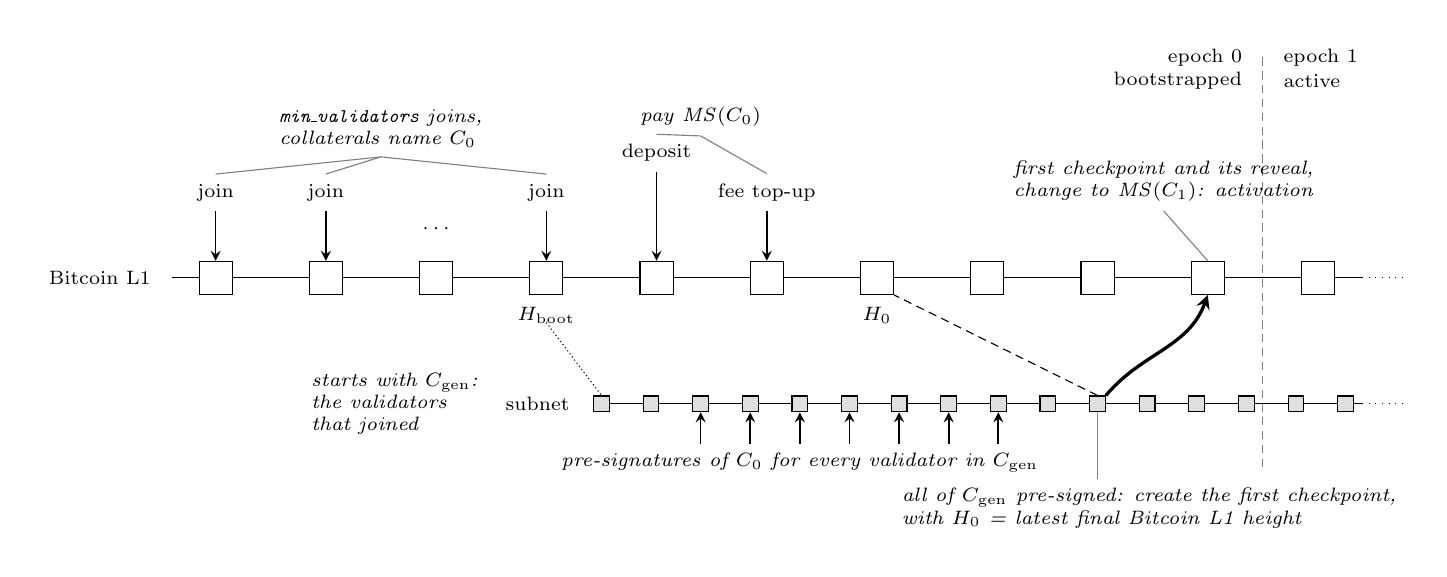
\begin{tikzpicture}[x=1.4cm, y=1cm, font=\scriptsize,
    show background rectangle, background rectangle/.style={fill=white},
    blk/.style={draw, fill=white, minimum width=0.42cm, minimum height=0.42cm, inner sep=0pt},
    sblk/.style={draw, fill=gray!25, minimum width=0.2cm, minimum height=0.2cm, inner sep=0pt},
    tx/.style={-stealth, semithick},
    remark/.style={font=\scriptsize\itshape, align=left},
    link/.style={gray, thin}]
  % Bitcoin L1 chain
  \draw (0.6,0) -- (11.4,0);
  \draw[dotted] (11.4,0) -- (11.8,0);
  \node[anchor=east] at (0.5,0) {Bitcoin L1};
  \foreach \i in {1,...,11} \node[blk] (b\i) at (\i,0) {};
  % Joins
  \draw[tx] (1,0.85) node[above] (j1) {join} -- (b1.north);
  \draw[tx] (2,0.85) node[above] (j2) {join} -- (b2.north);
  \node at (3,0.62) {$\cdots$};
  \draw[tx] (4,0.85) node[above] (jn) {join} -- (b4.north);
  \node[remark] (rj) at (2.5,1.9) {\texttt{min\_validators} joins,\\collaterals name $C_0$};
  \foreach \n in {j1,j2,jn} \draw[link] (rj.south) -- (\n.north);
  \node[below=1pt] at (b4.south) {$H_{\mathrm{boot}}$};
  % Deposits and fee top-ups
  \draw[tx] (5,1.35) node[above] (dp) {deposit} -- (b5.north);
  \draw[tx] (6,0.85) node[above] (ft) {fee top-up} -- (b6.north);
  \node[remark] (rd) at (5.4,2.05) {pay $\mathit{MS}(C_0)$};
  \draw[link] (rd.south) -- (dp.north);
  \draw[link] (rd.south) -- (ft.north);
  % H_0, activation and the epochs
  \node[below=1pt] at (b7.south) {$H_0$};
  \draw[densely dashed, gray] (10.5,2.8) -- (10.5,-2.4);
  \node[anchor=east] at (10.4,2.8) {epoch $0$};
  \node[anchor=west] at (10.6,2.8) {epoch $1$};
  \node[anchor=east] at (10.4,2.5) {bootstrapped};
  \node[anchor=west] at (10.6,2.5) {active};
  % Subnet chain
  \draw (4.5,-1.6) -- (11.4,-1.6);
  \draw[dotted] (11.4,-1.6) -- (11.8,-1.6);
  \node[anchor=east] (sl) at (4.3,-1.6) {subnet};
  \foreach \j in {0,...,15} \node[sblk] (s\j) at (4.5+0.45*\j,-1.6) {};
  \draw[densely dotted] (b4.south) ++(0,-0.35) -- (s0.north);
  \node[remark, anchor=east] at ([xshift=-3pt]sl.west) {starts with $C_{\mathrm{gen}}$:\\the validators\\that joined};
  % Pre-signatures collected on the subnet
  \foreach \j in {2,...,8} \draw[tx] ($(s\j.south)+(0,-0.4)$) -- (s\j.south);
  \node[remark, below] at (6.3,-2.1) {pre-signatures of $C_0$ for every validator in $C_{\mathrm{gen}}$};
  % First checkpoint: created at s10, under the Bitcoin L1 tip b9; H_0 = b7 is the latest final block
  \draw[densely dashed] (s10.north) -- (b7.south east);
  \draw[-stealth, very thick] (s10.north east) to[out=50, in=-110] (b10.south);
  \node[remark, anchor=north east] (rc) at (11.8,-2.55) {all of $C_{\mathrm{gen}}$ pre-signed: create the first checkpoint,\\with $H_0$ = latest final Bitcoin L1 height};
  \draw[link] (rc.north -| s10.south) -- (s10.south);
  \node[remark, anchor=south] (rf) at (9.6,0.85) {first checkpoint and its reveal,\\change to $\mathit{MS}(C_1)$: activation};
  \draw[link] (rf.south) -- (b10.north);
\end{tikzpicture}
\end{document}
